\documentclass{article}
\usepackage[T1,T2A]{fontenc}
\usepackage[utf8]{inputenc}
\usepackage[english,russian]{babel}

\usepackage[left=3cm,right=3cm,
    top=3cm,bottom=3cm,bindingoffset=0cm]{geometry}

\usepackage{graphicx}
\usepackage{color}
\usepackage{hyperref}
\usepackage{amsmath}
\usepackage{amsfonts}

\usepackage{setspace}
\usepackage{indentfirst}
\usepackage{textcomp}
\usepackage{ifthen}
\usepackage{calc}

\title{Теория Вероятностей и Математическая Статистика\\
ФИИТ, 2 курс, 4 семестр}
\author{Практика 5}

\begin{document}
\maketitle

%\begin{center}
%    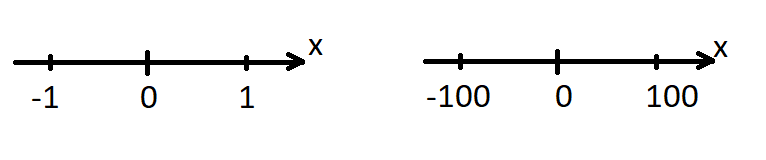
\includegraphics[scale=0.6]{9.png}
%\end{center}

\section{Задача 3.38 (ДЗ)}

Бросок монеты до серии ГГГ подряд. Какова вероятность того, что придется бросать ровно: а) 6 раз; б) 7 раз.
\\

а) 6 бросков. Распишем вариант подобного:

\begin{center}
* * Р Г Г Г\\
1 2 3 4 5 6
\end{center}

$$\rightarrow 1 \cdot 1 \cdot 1 \cdot \frac{1}{2}
\cdot \Bigl(\frac{1}{2}\Bigr)^3 = \frac{1}{16}$$
\\

б) 7 бросков. Так же распишем:

\begin{center}
$\overbrace{* * *}$ Р Г Г Г\\
1 2 3 4 5 6 7
\end{center}

Первые три монеты -- любая последовательность, кроме ГГГ:

$$\rightarrow \Bigl(1 - \frac{1}{8}\Bigr) \cdot \frac{1}{2} \cdot \frac{1}{8} =  \frac{7}{128} $$

\section{Задача 3.78}

Какова вероятность того, что при пяти бросаниях монеты герб выпадает по меньшей мере три раза подряд.
\\

Попробуем пронумероавть места и расставить последовательности ГГГ.

\begin{center}
$\underline{\text{\quad1 2 3 4 5 }}$\\
1) Г Г Г * * \\
2) * Г Г Г *\\
3) * * Г Г Г
\end{center}

Можно заметить, что наши варианты пересекаются. Допустим, для второго варианта на первом месте поставим Г, и получим снова первый вариант. Поэтому добавим некоторые ограничения на наши варианты:

\begin{center}
$\underline{\text{\quad1 2 3 4 5 }}$\\
1) Г Г Г * * \\
2) Р Г Г Г *\\
3) * Р Г Г Г
\end{center}

Тогда получим следующие вероятности:

1) $\rightarrow \frac{1}{8} \cdot 1^2 $

2) $\rightarrow \frac{1}{2} \cdot \frac{1}{8} \cdot 1$

3) $\rightarrow 1 \cdot \frac{1}{2} \cdot \frac{1}{8} $

Больше вариантов вроде как нет, так что итоговая вероятность будет суммой $\sum = \frac{1}{4}$

\section{Задача A}
Бросают 7 монет. Найдите вероятность того, что при этом выпадет 3 герба.
\\

В данном случае имеет место \textbf{схема Бернулли}. У нас в каждом испытании реализуется либо Герб, либо Решка. Каждый вариант достигается с вероятностью $\frac{1}{2}$. Тогда:

$$P_7(3) = C_7^3 \cdot \Bigl(\frac{1}{2}\Bigr)^3 \cdot \Bigl(\frac{1}{2}\Bigr)^{7 - 3}
= \frac{7 \cdot 6 \cdot 5}{6} \cdot \frac{1}{2^7}$$

\section{Задача B}
Монету бросают до тех пор, пока герб будет зафиксирован в третий раз. Найдите в-ть того, что монету потребуется бросать 7 раз.
\\

Можно зафиксировать Герб на седьмой позиции (так как бросам до 7 раз). Оставшиеся 6 мест заполняем двумя Гербами и остальными Решками. Таким образом, мы делим наши исходы на две части -- первые 6 бросков (где должно быть 2 Герба) и последний бросок с выпадением Герба:

\begin{center}
    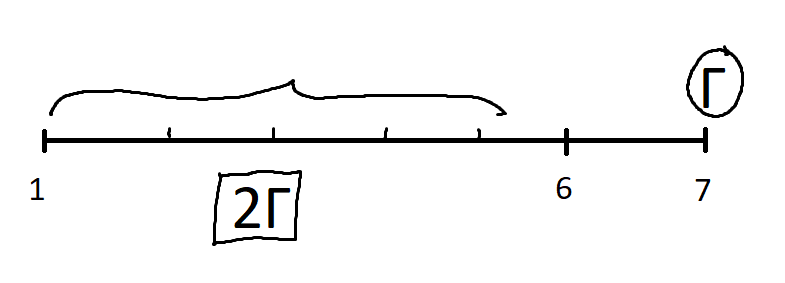
\includegraphics[scale=0.35]{1.png}
\end{center}

$$P = \Biggl(C_6^2 \Bigl(\frac{1}{2}\Bigr)^2 \Bigl(\frac{1}{2}\Bigr)^{6 - 2}\Biggr)\cdot\frac{1}{2} = \ldots$$

\section{Задача C}

Монету бросают до тех пор, пока герб будет зафиксирован в третий раз. Найдите в-ть того, что для этого хватит 7 бросков.
\\

Казалось бы, та же задача, но вместо фиксированного количества бросков мы имеем переменное количество от 3 до 7.

Таким образом, наши варианты -- с 3, 4, 5, 6 и 7 бросками:



\begin{center}
\begin{tabular}{ l l | l}
\underbrace{1 2 3} &  & $P_3 = \frac{1}{2}^3$\\
\text{ }3г &  &\\
\\

\underbrace{1-3} & 4 & $P_4 = C_3^2 \cdot \frac{1}{8}\cdot \frac{1}{2}$\\
\text{ }2г & г &\\
\\

\underbrace{1-4} & 5 & $P_5 = C_4^2 \cdot \frac{1}{16}\cdot \frac{1}{2}$\\
\text{ }2г & г &\\
\\

\underbrace{1-5} & 6 & $P_6 = C_5^2 \cdot \frac{1}{32}\cdot \frac{1}{2}$\\
\text{ }2г & г &\\
\\

\underbrace{1-6} & 7 & $P_7 = C_6^2 \cdot \frac{1}{64}\cdot \frac{1}{2}$\\
\text{ }2г & г &\\
\\
\end{tabular}
\end{center}

Так как вероятности несовместны, мы их можем просто просуммировать и получить ответ.

\section{Задача D}
Бросают 7 монет. Найдите вероятность того, что при этом выпадет 3 герба, ЕСЛИ герб выпал не на всех монетах.
\\

Ключевое слово в этой задаче -- "если". Тогда мы получаем задачу два события $A$ и $B$ и условную вероятность $\rightarrow P(A|B) = \frac{P(AB)}{P(B)}$. Распишем эти события:

$A = \{$ выпало 3 Герба из 7 $\}$

$B = \{$ Герб выпал не на всех монетах $\}$

Кстати, $AB = A$. Событие $A$ входит в событие $B$. Так что фактически (после сокращений) нам нужно найти отношение двух вероятностей:

$$\frac{P(A)}{P(B)} = \frac{C_7^3 \cdot \frac{1}{128}}{1 - \frac{1}{128}} = \ldots$$

\section{Задача 5.40}

Подбрасывают три игральные кости. Какова вероятность того, что проиведение всех выпавших цифр будет равно: а) 20; б) 24?
\\

a) Чтобы получилось такое произведение ($20$), у нас должны выпать следующе значения:  $(1, 4, 5)$, $(2, 2, 5)$.

Пронумеруем наши возможные выпадения $[1, 2, 3, 4, 5, 6]$ и распишем вероянтности выбранных произведений по полиномиальной формуле (n опытов == 3):

$$(1, 4, 5) \rightarrow P_3(1, 0, 0, 1, 1, 0) = \frac{3!}{(1!)^3\cdot(0!)^3}\cdot \Bigl(\frac{1}{6}\Bigr)^3$$

$$(2, 2, 5) \rightarrow P_3(0, 2, 0, 0, 1, 0) = \frac{3!}{2!\cdot 1!\cdot(0!)^4}\cdot \Bigl(\frac{1}{6}\Bigr)^3$$

Так как сообытия несовместны, достаточно найти сумму вероятностей.
\\

б) Для произведения $24$ достаточно проделать те же операции, то есть расписать возможные произведения (их 3 шт.) и найти вероятности.

\section{Задача 5.10}

Каждый выпущенный по цели снаряд попадает в нее, независимо от других снарядов, с вероятностью $0.4$.

Если в цель попал один снаряд, она поражается с вероятностью $0.3$; если два снаряда, -- с вероятностью $0.7$; если три или более снарядов, то цель поражается наверняка.

Найдите вероятность поражения цели при условии, что по ней выпущено: а) 3 снаряда; б) 4 снаряда.
\\

Попробуем расписать два действия:

\quad1) попадание \qquad\qquad 2) поражение \qquad\qquad$\Rightarrow$ формула полной вероятности.
\\

Распишем гипотезы:

\qquad$H_0 = \{$ 0 попаданий $\}$

\qquad$H_1 = \{$ 1 попаданий $\}$

\qquad$H_2 = \{$ 2 попаданий $\}$

\qquad$H_3 = \{$ 3 попаданий $\}$

\qquad$H_4 = \{$ 4 попаданий $\}$
\\

И условные вероятности:

$\qquad P(A | H_0) = 0 \qquad P(A|H_1) = 0.3 \qquad P(A|H_2) = 0.7 \qquad P(A|H_3) = P(A|H_4) = 1$
\\

Таким образом, вероятность поражения цели можно найти по формуле полной вероятности:

$$P(A) = \sum\limits_{k = 0}^4 P(H_k) \cdot P(A|H_k) = \ldots$$

\section{Контрольная}

На следующей лекции (19.03.21) будет мини-контрольная по разделу "Случайные события" со следующими критериями оценивания:

\begin{center}
    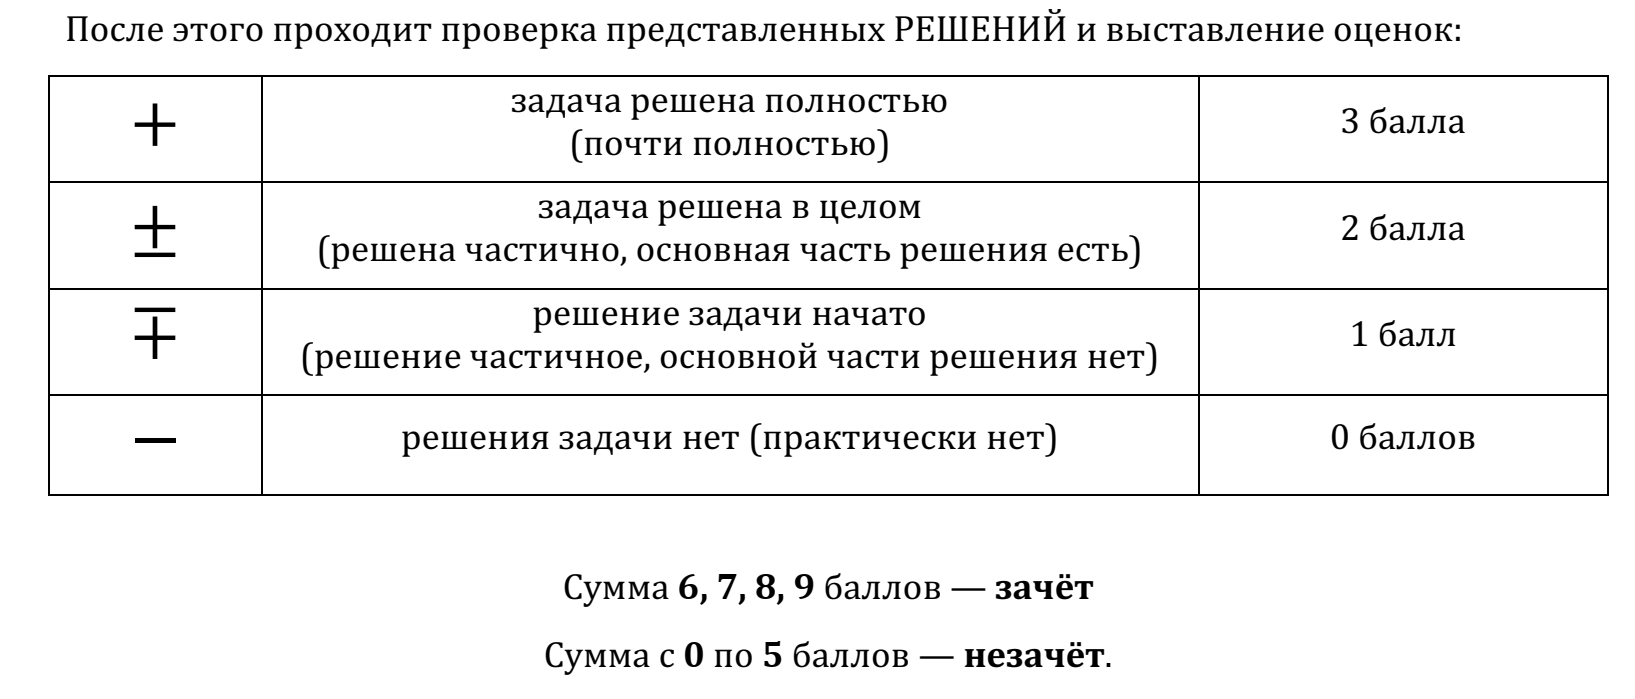
\includegraphics[scale=0.25]{Критерии.png}
\end{center}

Задачи распределяются по этим темам:

\quad 1. классическая схема

\quad 2. сложение, умн. вероятностей или формула полн. вер-ти

\quad 3. бернулли, полиномиальная
\\

Также стоит выполнить задачи электронного учебника в параграфах 1 и 3. Это поможет повысить оценку контрольной (ненулевую) в случае чего.

\end{document}
